\section{Control de datos faltantes}
Se reconstruyó el calendario diario completo de 1981--2022, incluidos los años
bisiestos. De 15\,340 días esperados, el archivo contiene 15\,085 fechas y omite
255 días (1,66\,\%) tanto en P como en Q. Son las mismas fechas ausentes para
ambas variables: no se deben sumar como 510 días distintos.

\subsection{Criterio de completitud}
Se exige el 100 \% de días válidos para que la lluvia acumulada y el caudal medio representen el mes completo, evitando presentar sumas parciales de lluvia como totales mensuales. Este mismo criterio se mantiene en los análisis de CHIRPS y caudal; R conserva los mismos meses válidos que Q porque se calcula a partir de él.

Se retiene únicamente un mes con el 100\,\% de sus días válidos. De 504 meses,
se conservan 485 (96,23\,\%) y se excluyen 19 (3,77\,\%): seis totalmente ausentes
y trece parcialmente completos. Los ceros se conservan y los faltantes permanecen
como vacíos; no se rellena ni se prorratea la precipitación.

\begin{figure}[H]
\centering
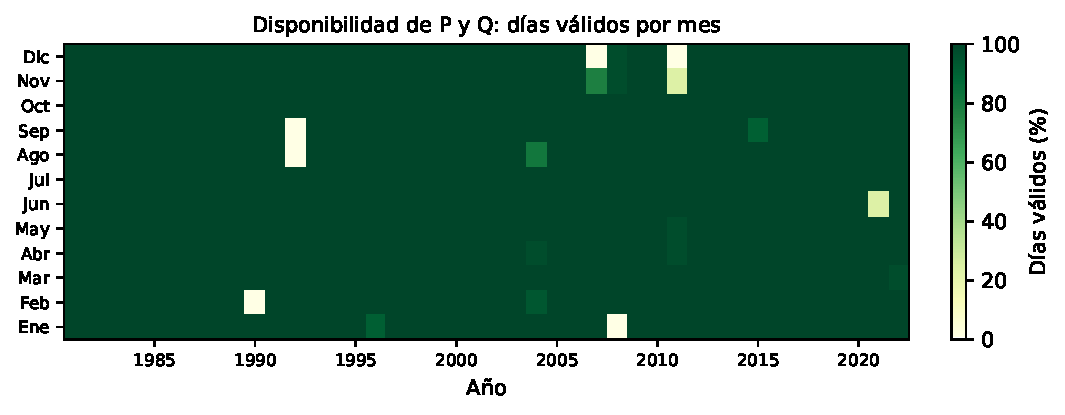
\includegraphics[width=\linewidth]{figuras/control_faltantes.pdf}
\caption{Disponibilidad diaria dentro de cada mes. P y Q tienen la misma cobertura
en el archivo CAMELS; 100\,\% indica un mes completo.}
\label{fig:faltantes}
\end{figure}

\begin{center}
\small
\begin{tabular}{lrrrr}
\hline
Mes & Esperados & Válidos P/Q & Faltantes P/Q & Completitud (\%) \\
\hline
1990-02 & 28 & 0 & 28 & 0,00 \\
1992-08 & 31 & 0 & 31 & 0,00 \\
1992-09 & 30 & 0 & 30 & 0,00 \\
1996-01 & 31 & 28 & 3 & 90,32 \\
2004-02 & 29 & 27 & 2 & 93,10 \\
2004-04 & 30 & 29 & 1 & 96,67 \\
2004-08 & 31 & 25 & 6 & 80,65 \\
2007-11 & 30 & 23 & 7 & 76,67 \\
2007-12 & 31 & 0 & 31 & 0,00 \\
2008-01 & 31 & 0 & 31 & 0,00 \\
2008-11 & 30 & 29 & 1 & 96,67 \\
2008-12 & 31 & 30 & 1 & 96,77 \\
2011-04 & 30 & 29 & 1 & 96,67 \\
2011-05 & 31 & 30 & 1 & 96,77 \\
2011-11 & 30 & 7 & 23 & 23,33 \\
2011-12 & 31 & 0 & 31 & 0,00 \\
2015-09 & 30 & 27 & 3 & 90,00 \\
2021-06 & 30 & 7 & 23 & 23,33 \\
2022-03 & 31 & 30 & 1 & 96,77 \\
\hline
\end{tabular}
\end{center}

\subsection{Consecuencias para la interpretación}
Los vacíos continuos más largos son diciembre de 2007--enero de 2008 (62 días),
agosto--septiembre de 1992 (61 días) y 8 de noviembre--31 de diciembre de 2011
(54 días). No es posible reconstruir su evolución a partir del archivo analizado;
los faltantes pueden sesgar la representación de temporadas y extremos.

Como sensibilidad, aceptar meses de Q con al menos 90\,\% de días elevaría la
muestra a 494 meses y la media a 100,91~m$^3$/s, frente a 98,70~m$^3$/s con el
criterio estricto. Se mantiene el 100\,\% como resultado principal. Esta comparación
no justifica tratar sumas parciales de precipitación como acumulados completos.

Este control describe el archivo CAMELS ensamblado, no la disponibilidad original
de CHIRPS, IMERG ni de las estaciones pluviométricas individuales. No se supone
que los faltantes ocurran al azar.

% CONCLUSION_COMPROBACION_INICIO
\subsection{Conclusión de la comprobación de datos}
Durante la comprobación de las series revisadas no se encontraron inconsistencias en las fechas, duplicados, unidades ni valores negativos de lluvia, caudal o escorrentía. No fue necesario corregir datos por estos criterios. Sin embargo, los archivos tabulares revisados de CAMELS y lluvia local no incluyen banderas explícitas de calidad, lo que limita la validación y no permite garantizar la exactitud de todos los valores.
% CONCLUSION_COMPROBCACION_FIN



% CONCLUSION_RECONSTRUCCIONES_INICIO
\subsection{Conclusión sobre reconstrucciones y estimaciones}
\textbf{Reconstrucción del calendario y ajuste de la geometría de las celdas:} se completaron las fechas y se ajustaron los límites de las celdas IMERG, sin rellenar los vacíos ni modificar los valores originales.

\textbf{Estimaciones de modelos y escenario hipotético P95:} se generaron valores para evaluar los modelos del punto 2 y la influencia de los extremos. Estos resultados permanecen separados y no sustituyen ni rellenan los datos originales.
% CONCLUSION_RECONSTRUCCIONES_FIN
